\chapter{Ovládání aplikace}

\section{Aplikace}

Ovládání aplikace by mělo být intuitivní. V hlavním menu jsou volby Nová hra, Změnit hru, Nastavení a Dávkové spouštění. Nová hra restartuje hru s novým nastavením. Ve změnit hru lze vybrat jednu ze tří implementovaných her a v Nastavení ji nakonfigurovat.

Menu Dávkové spouštění slouží k provádění experimentů. Zpět z Dávkového spouštění se uživatel dostane vybráním Nová hra z hlavní nabídky.


\begin{figure}
  \centering
  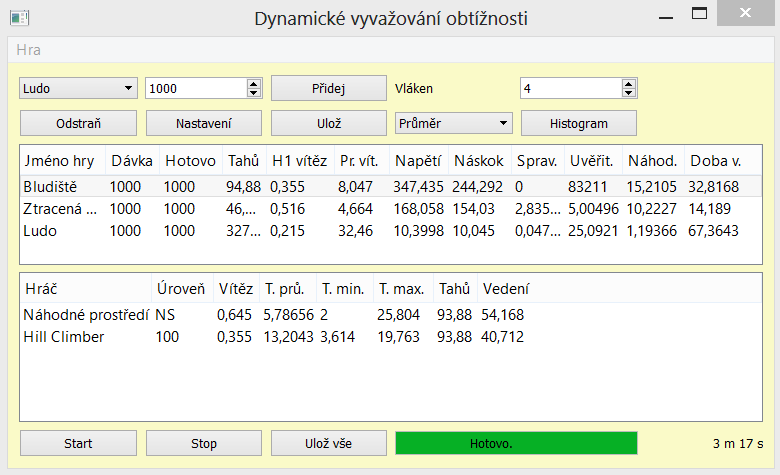
\includegraphics[width=0.90\textwidth]{appdavka}
	\caption{Uživatelské rozhraní dávkového spouštění experimentů. }
	\label{fig-appdavka}
\end{figure}

Uživatel přidá novou dávku zvolením dvou parametrů. Z výběrového menu vybere hru a nastaví počet iterací experimentu. Tlačítkem Přidej vytvoří jeden nový experiment, který se objeví v seznamu navolených experimentů. 

Po označení experimentu v seznamu může uživatel využívat čtveřici tlačítek Odstraň, Nastavení, Ulož, Histogram. Odstraň vymaže experiment z dávky, Nastavení spustí nastavení pro hru, Ulož umožňuje uložit výsledky proběhlého experimentu, Histogram otevře okno, v kterém lze zobrazit jednotlivé metriky pro jeden experiment jako histogram. Dále je ve stejném řádku možnost voleb Průměr, Směrodatná odchylka, Minimum a Maximum. Dle volby se po proběhnutí experimentů v jejich seznamu zobrazují příslušné hodnoty z daných experimentů. 


\begin{figure}
  \centering
  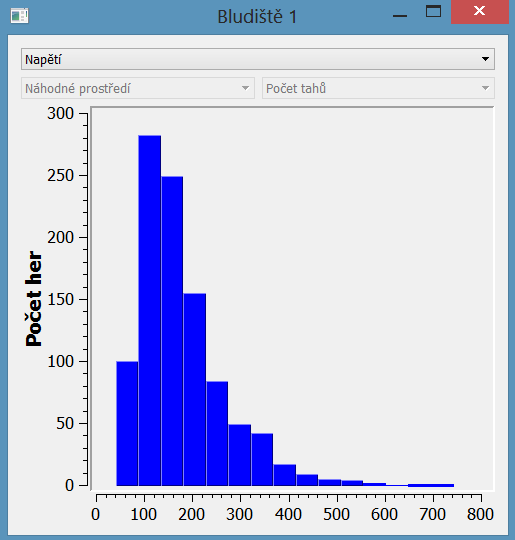
\includegraphics[width=0.75\textwidth]{apphistogram}
	\caption{Histogram metriky Napětí pro hru bludiště a 1000 iterací experimentu. }
	\label{fig-apphistogram}
\end{figure}

Pomocí tlačítka Start se spustí navolené experimenty jeden za druhým. Iterace v rámci jednoho experimentu se rozdělí do předem definovaného počtu vláken. Tlačítkem Stop se experimenty zastaví, ale nechají se doběhnout aktuálně rozehrané hry. Pomocí tlačítka Uložit vše lze hromadně uložit výsledky všech experimentů do zvolené složky. 

V průběhu experimentu se zobrazuje uplynulý čas a velice hrubý odhad skončení experimentů. Spočítá se dle průměrné doby na jednu iteraci od začátku spuštění experimentů a dle počtu zbylých iterací ve všech experimentech.

Po označení experimentu v seznamu se zároveň zobrazí ve spodním okně několik metrik k jednotlivým hráčům. Pro každého hráče je uvedeno jeho jméno, úroveň, poměr vítězství. T. prů. T. min., T. max. značí průměrný, minimální a maximální počet tahů hráče během hry. Poslední dvě metriky znamenají kolikrát byl hráč na tahu a kolik kol byl ve vedení.

V seznamu experimentů se zobrazuje jméno hry, celkový a proběhlý počet iterací experimentu, celkový počet tahů, poměr vítězství prvního hráče a metriky prohození vítězů, Napětí, Náskok, Spravedlnost, Uvěřitelnost, Náhodnost, Doba vedení v tomto pořadí.

\section{Hry}

V této části stručně popíši uživatelské rozhraní jednotlivých her. Nezmiňuji zde pravidla her, která byla uvedena v páté kapitole.

Nastavení her je stejné pro dávkové spouštění i při hraní člověk proti počítači. V levé polovině uživatel může nastavit algoritmy pro jednotlivé hráče a případně jejich úroveň, pokud to daný algoritmus umožňuje. Pod nastavením hráčů jsou speciální nastavení pro jednotlivé hry popsány níže.

V pravé části nastavení se volí hráč prostředí a koeficienty pro jednotlivé metriky. Nastavení se stane platné až po uložení tlačítkem Uložit.

\subsection{Bludiště}

Hra se ovládá pomocí levého tlačítka myši. Hráč ovládá žlutou kuličku a snaží se dostat včas ke všem bombám, které jsou na mapě znázorněny zelenými čtverci. Hráč vždy kliknutím vybere, které další dveře se mají otevřít. K otevřeným dveřím postava dojde skokem. Dveře jsou znázorněny oranžovými, modrými a červenými čtverci. Dle barvy dveří a jejich vzdálenosti od předchozí pozice, se hráči odečtou zbývající kroky do konce hry.

\begin{figure}
  \centering
  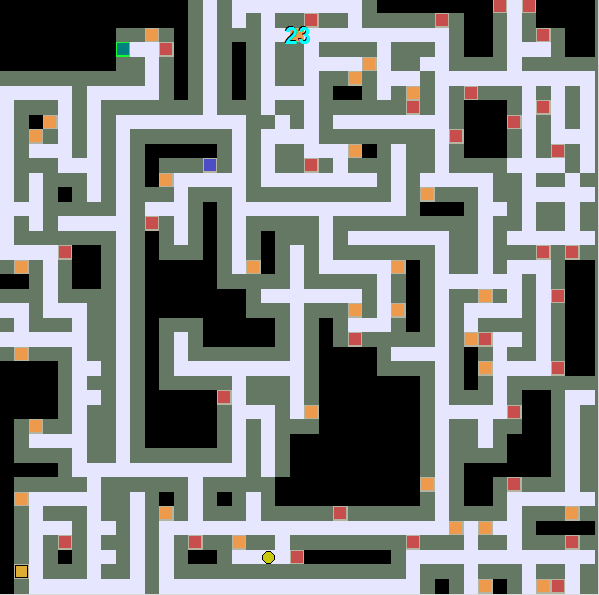
\includegraphics[width=0.75\textwidth]{appmaze}
	\caption{Uživatelské rozhraní hry Bludiště. Zelený čtverec představuje možnou bombu. }
	\label{fig-appmaze}
\end{figure}

Zbývající počet kroků do konce hry zobrazuje tyrkysové číslo v horní části hry. 

V případě, že některá bomba se stane nedostupnou, tak byla falešná a zmizí z mapy.

\emph{Speciální nastavení} : Před hrou hráč může upravit parametry velikosti bludiště a počáteční limit na počet kroků.

\subsection{Ludo}

Hra Ludo se také ovládá pomocí myši. Kostkou se hází automaticky. Hodnota, která padla, je znázorněna uprostřed herní plochy. Hráč může pohnout s figurami, které jsou na bíle zvýrazněném poli. Jestliže figurkou nemůže pohnout, tak buď mu v tom brání vlastní figurka, kterou by jinak vyhodil, nebo je před figurkou již obsazené bezpečné místo.

\begin{figure}
  \centering
  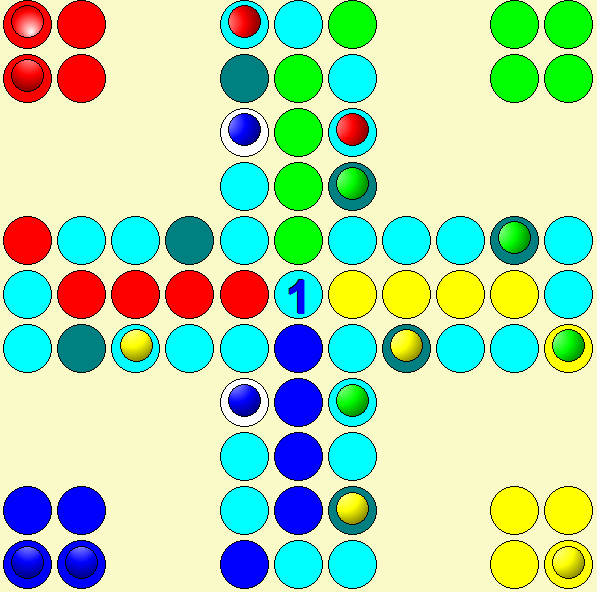
\includegraphics[width=0.75\textwidth]{appludo}
	\caption{Uživatelské rozhraní hry Ludo. Bílý podklad značí aktivní figurky. }
	\label{fig-appludo}
\end{figure}

Bezpečná místa jsou zvýrazněna tmavší barvou.

V případě, že hráč nemá ani jednu figurkou na hlavním plánu, hází kostkou až třikrát. Pouze první hod se provede automaticky, ostatní hody provádí hráč kliknutím doprostřed herního pole.

\emph{Speciální nastavení} : Lze nastavit hru pouze dvou hráčů. V tom případě se ignoruje nastavení druhého a čtvrtého hráče.

\subsection{Ztracená města}

Hra se opět ovládá pouze pomocí levého tlačítka myši. Každý tah se vždy skládá ze třech kliknutí. Prvním kliknutím na kartu v ruce hráč vybere, s kterou kartou bude hrát. 

Při druhém kliknutí hráč vybírá, co s kartou udělá. Může jí buď zahodit vybráním příslušného odkládacího balíčku, které jsou na začátku hry znázorněny šedivým čtvercem se zaoblenými hranami. V případě, že kartu může zahrát, klikne pod odkládací balíček dané barvy. 


\begin{figure}
  \centering
  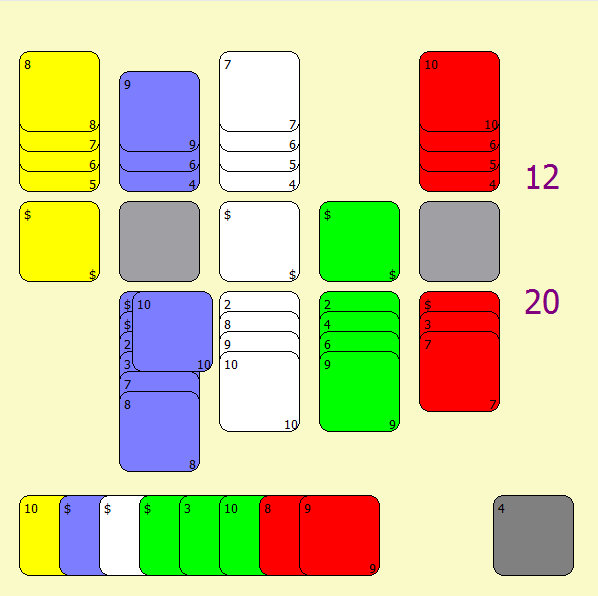
\includegraphics[width=0.75\textwidth]{applc}
	\caption{Uživatelské rozhraní hry Ztracená města. }
	\label{fig-applc}
\end{figure}

Nakonec třetím kliknutím hráč vybere, odkud dobere kartu. Jedna z možností je dobrat z dobíracího balíčku, který je znázorněn šedivě v pravém dolním rohu. Je na něm číslo udávající počet zbývajících karet v balíčku. V případě, že jsou na stole odložené karty, může hráč kliknout na jednu z nich a vzít si ji do ruky.

Hráčovi se vždy zvýrazňují oblasti ve hře, které jsou zrovna aktivní a hráč na ně může kliknout.

\emph{Speciální nastavení} : Lze nastavit počet karet v ruce. Oficiální pravidla hry umožňují variantu 8 a 5 karet v ruce.

\endinput
%%
%% End of file `ch01.tex'.
